\section{Instrument Accuracy Test} \label{subsec:8_1_AccTest}
The instrument was not tested for the full bandwidth of the desigend front end, due to time constraints. The proper test equipment was also not available to properly perform this test. The test results from appendix \refq{App:AccuracyBWTest} have been plotted and can be compared with the requirements seen on figure \refq{fig_5_ModulusAccuracy} and figure \refq{fig_5_PhaseAccuracy} in section \refq{ch:SystemRequirements} regarding the instruments modulus and phase accuracy.

A true metrology grade laboratory with precise known standards is required to properly test the developed system. This was not available at the time, thus the instrument has been tested against assumed stable film resistors, PP capacitors and a single inductor.

appendix \refq{App:AccuracyBWTest} shows the various impedances that the system has been compared with. The tests conducted in section \refq{subsec:ModulusAccuracyTest_res} in said appendix can be used to generate the following plots. 

Figure \refq{fig_8_ModulusAccuracy} shows observed test error for modulus accuracy, the requirement for modulus accuracy as per section \refq{ch:SystemRequirements} and the R\&S LCX-200 specification for the same measurement as the test performes.

Figure \refq{fig_8_ArgumentAccuracy} shows the same but for argument.


\begin{figure}[H]
    \centering
    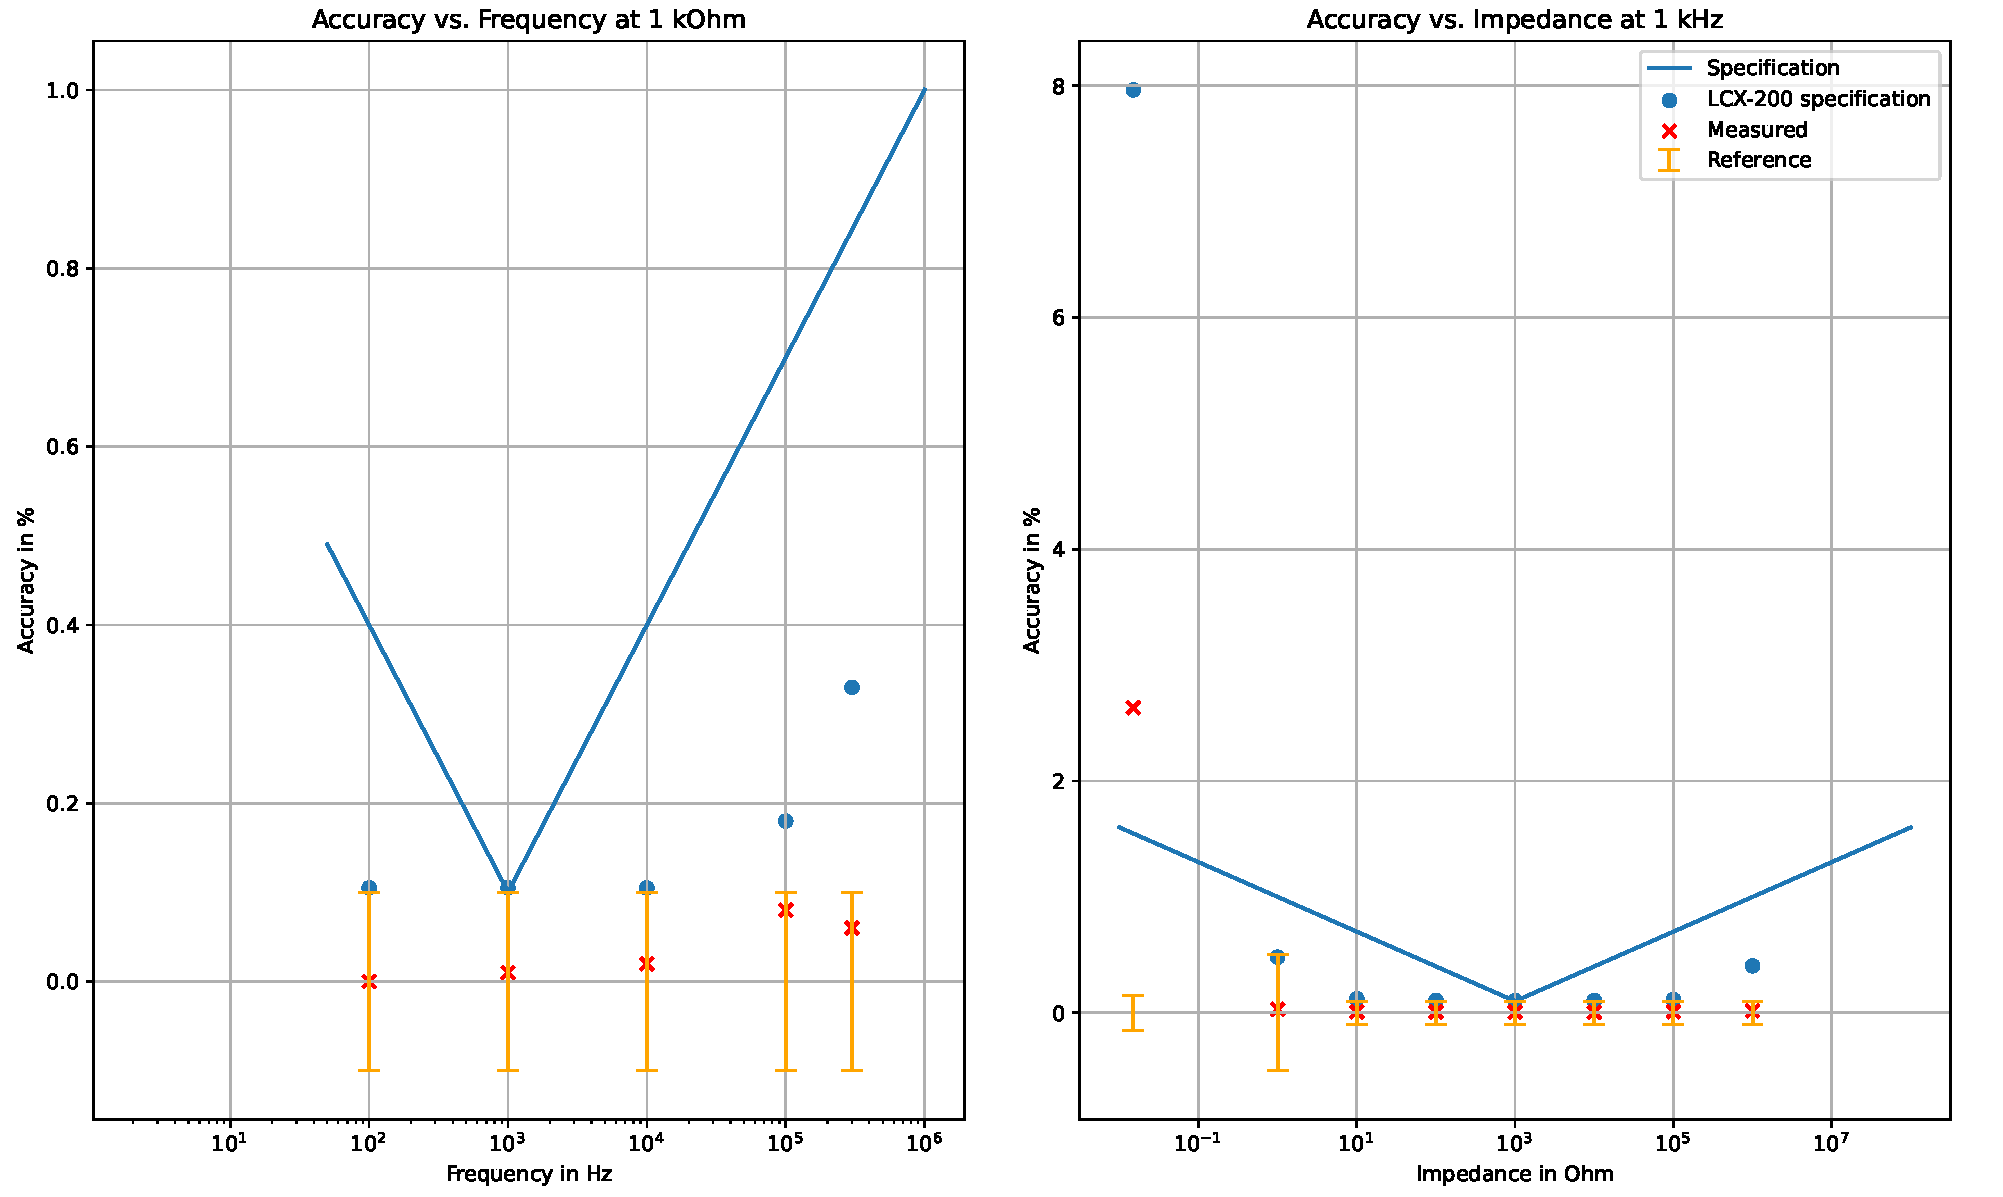
\includegraphics[width=1\textwidth]{Sections/8_SystemVerification/Figures/SpecVTest.pdf}
    \caption{Plots of the requirement for modulus accuracy, left for fixed impedance, but varying frequency, right with fixed frequency but varying impedance. The dots are the specifications of the R\&S LCX-200, with the \SIQ{1}{\mega\hertz} option. The requirements are from section \refq{ch:SystemRequirements}. The errorbars are the manufacturer specified tolerances.}
    \label{fig_8_ModulusAccuracy}
\end{figure}
  

\begin{figure}[H]
    \centering
    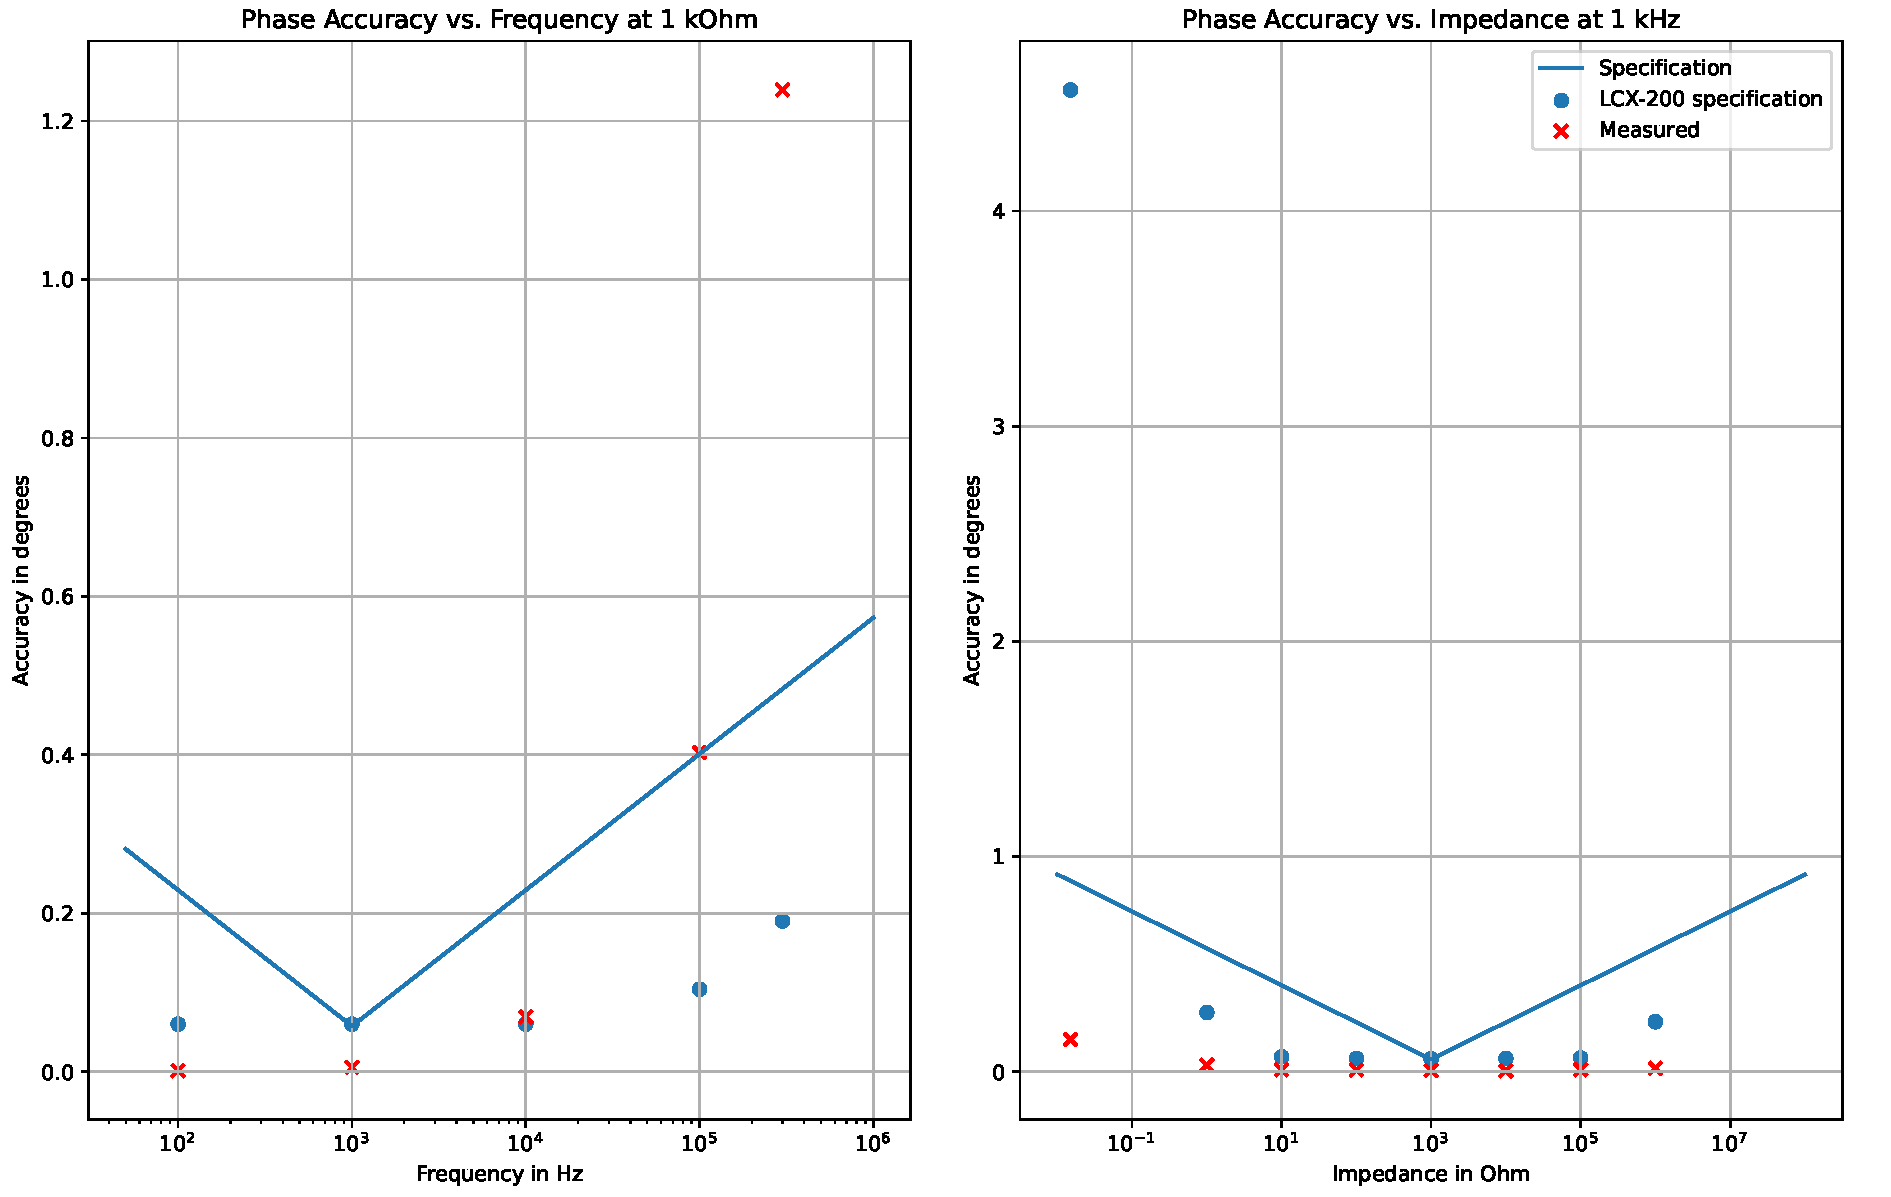
\includegraphics[width=1\textwidth]{Sections/8_SystemVerification/Figures/SpecVTest_Phase.pdf}
    \caption{Plots of the requirement for argument accuracy, left for fixed impedance, but varying frequency, right with fixed frequency but varying impedance. The dots are the specifications of the R\&S LCX-200, with the \SIQ{1}{\mega\hertz} option. The requirements are from section \refq{ch:SystemRequirements}.}
    \label{fig_8_ArgumentAccuracy}
\end{figure}
  
One thing to take note of here is that the only magnitude measurement that is not within said requirement is at \SIQ{15}{\milli\ohm}. It should however be noted that the R\%S LCX-200 specifes \SIQ{8}{\%} at such a low value. The measured phase angle is observed to accurate to within the requirement to around \SIQ{10}{\kilo\hertz}. At higher frequencies a rather large phase error seems to be introduced. The modulus Accuracy does hoever not seem to degrade much with frequency, indicating that the phase error might be due to an incorrect open/short correction model.
%Tilføjet grafer der viser faktisk præcision og sammenlign med graferne for modules og phase præcision i Requirements afsnittet. Evt læg dem oven i hinanden.